\chapter{Aufbereiten von Unterrichtsinhalten}\label{Aufbereitung}

\section{Didaktische Analyse nach Klafki / Kritisch-konstruktive Didaktik}

Die Didaktische Analyse ist ein zentrales Konzept der Unterrichtsplanung, entwickelt von Wolfgang Klafki.\footnote{Klafki, Wolfgang: Didaktische Analyse als Kern der Unterrichtsvorbereitung in: Roth, H. / Blumenthal, A. (Hg): Grundlegende Aufs\"{a}tze aus der Zeitschrift Die Deutsche Schule, Hannover 1964; Klafki, Wolfgang: Die bildungstheoretische Didaktik im Rahmen kritisch - konstruktiver Erziehungswissenschaft - oder: Zur Neufassung der Didaktischen Analyse in: Gudjons, H.: Didaktische Theorien / Westerrnanns P\"{a}dagogische Beitr\"{a}ge, Braunschweig 1986; Jank, W. / Meyer, H.: Didaktische Modelle, Frankfurt am Main 1991} Sie dient dazu, den Bildungsgehalt eines Themas systematisch zu untersuchen und die Unterrichtsgestaltung darauf aufzubauen. Klafkis Ansatz stellt die Frage in den Mittelpunkt, welchen Bildungswert ein Thema f\"{u}r die Lernenden hat.
\bip
Klafki identifiziert f\"{u}nf Grundfragen, die eine didaktische Analyse leiten:
\begin{enumerate}
\item{\textbf{Exemplarische Bedeutung:} Welches allgemeine Prinzip oder welche grundlegende Erkenntnis kann durch das Thema vermittelt werden?}
\item{\textbf{Gegenwartsbedeutung:} Welche Relevanz hat das Thema f\"{u}r die aktuelle Lebenswelt der Lernenden?}
\item{\textbf{Zukunftsbedeutung:} Welche Bedeutung hat das Thema f\"{u}r die zuk\"{u}nftige Entwicklung und Lebensbew\"{a}ltigung der Lernenden?}
\item{\textbf{Sachstruktur:} Wie ist der inhaltliche Aufbau des Themas und welche grundlegenden Zusammenh\"{a}nge m\"{u}ssen verstanden werden?}
\item{\textbf{Zug\"{a}nglichkeit:} Wie kann das Thema so aufbereitet werden, dass es f\"{u}r die Lernenden verst\"{a}ndlich und nachvollziehbar ist?}
\end{enumerate}

\bip

Die Didaktische Analyse nach Klafki zielt darauf ab, Unterrichtsinhalte so auszuw\"{a}hlen und zu gestalten, dass sie sowohl aktuelle als auch zuk\"{u}nftige Bildungsprozesse der Lernenden unterst\"{u}tzen. Dabei wird das Thema in einen gr\"{o}{\ss}eren Bildungszusammenhang gestellt, um nicht nur Wissen zu vermitteln, sondern auch die Selbst- und Weltverst\"{a}ndnis der Sch\"{u}ler zu f\"{o}rdern.

\bip

Es sei angemerkt, dass durch den Lehrplan, insbesondere der im Fach Physik, bereits eindeutig festgelegt ist, welche Themen in die Unterrichtsplanung einzubeziehen sind. Eine didaktische Analyse dieser Themen darf gern zu \"{U}bungszwecken versucht werden, aber eine Entscheidung bez\"{u}glich einer Themenauswahl ist nicht erforderlich.

\bip\bip
\section{Elementarisierung und didaktische Rekonstruktion}

\begin{ziele}
	Am Ende dieses Abschnitts können Sie\dots
	\begin{itemize}
		\item Elementarisierungsstufen angeben und hinsichtlich des Grades der Elementarisierung differenzieren.
		\item Gütekriterien für Elementarisierungen angeben und anhand eines Beispiels veranschaulichen.
		\item drei Elementarisierungstypen anhand eines Beispiels erläutern.
		\item einen fachwissenschaftlichen Inhalt für eine gegebene Zielgruppe elementarisieren
		\item Elementarisierungen in gegebenen Lernumgebungen benennen und hinsichtlich ihrer Grenzen analysieren.
	\end{itemize}	
\end{ziele}

\subsection{Elementarisierung}\label{Elementarisierung}

\begin{uea}
	Betrachten Sie folgende Darstellungen des Induktionsgesetzes:
	\begin{enumerate}
		\item $U = \dv{t} \int\limits_{A(t)} \vec{B}\cdot \dd{\vec{A}}$
		\item In einer durch ein Magnetfeld bewegten Leiterschleife wird eine Spannung induziert.
		\item Ist das Magnetfeld 2, 3, \dots, n mal so groß, so ist auch die induzierte Spannung 2, 3, \dots, n mal so groß.
		\item $U=B_0 L v$
		\item $\nabla\times\vec{E} = - \pdv{\vec{B}}{t}$
		\item 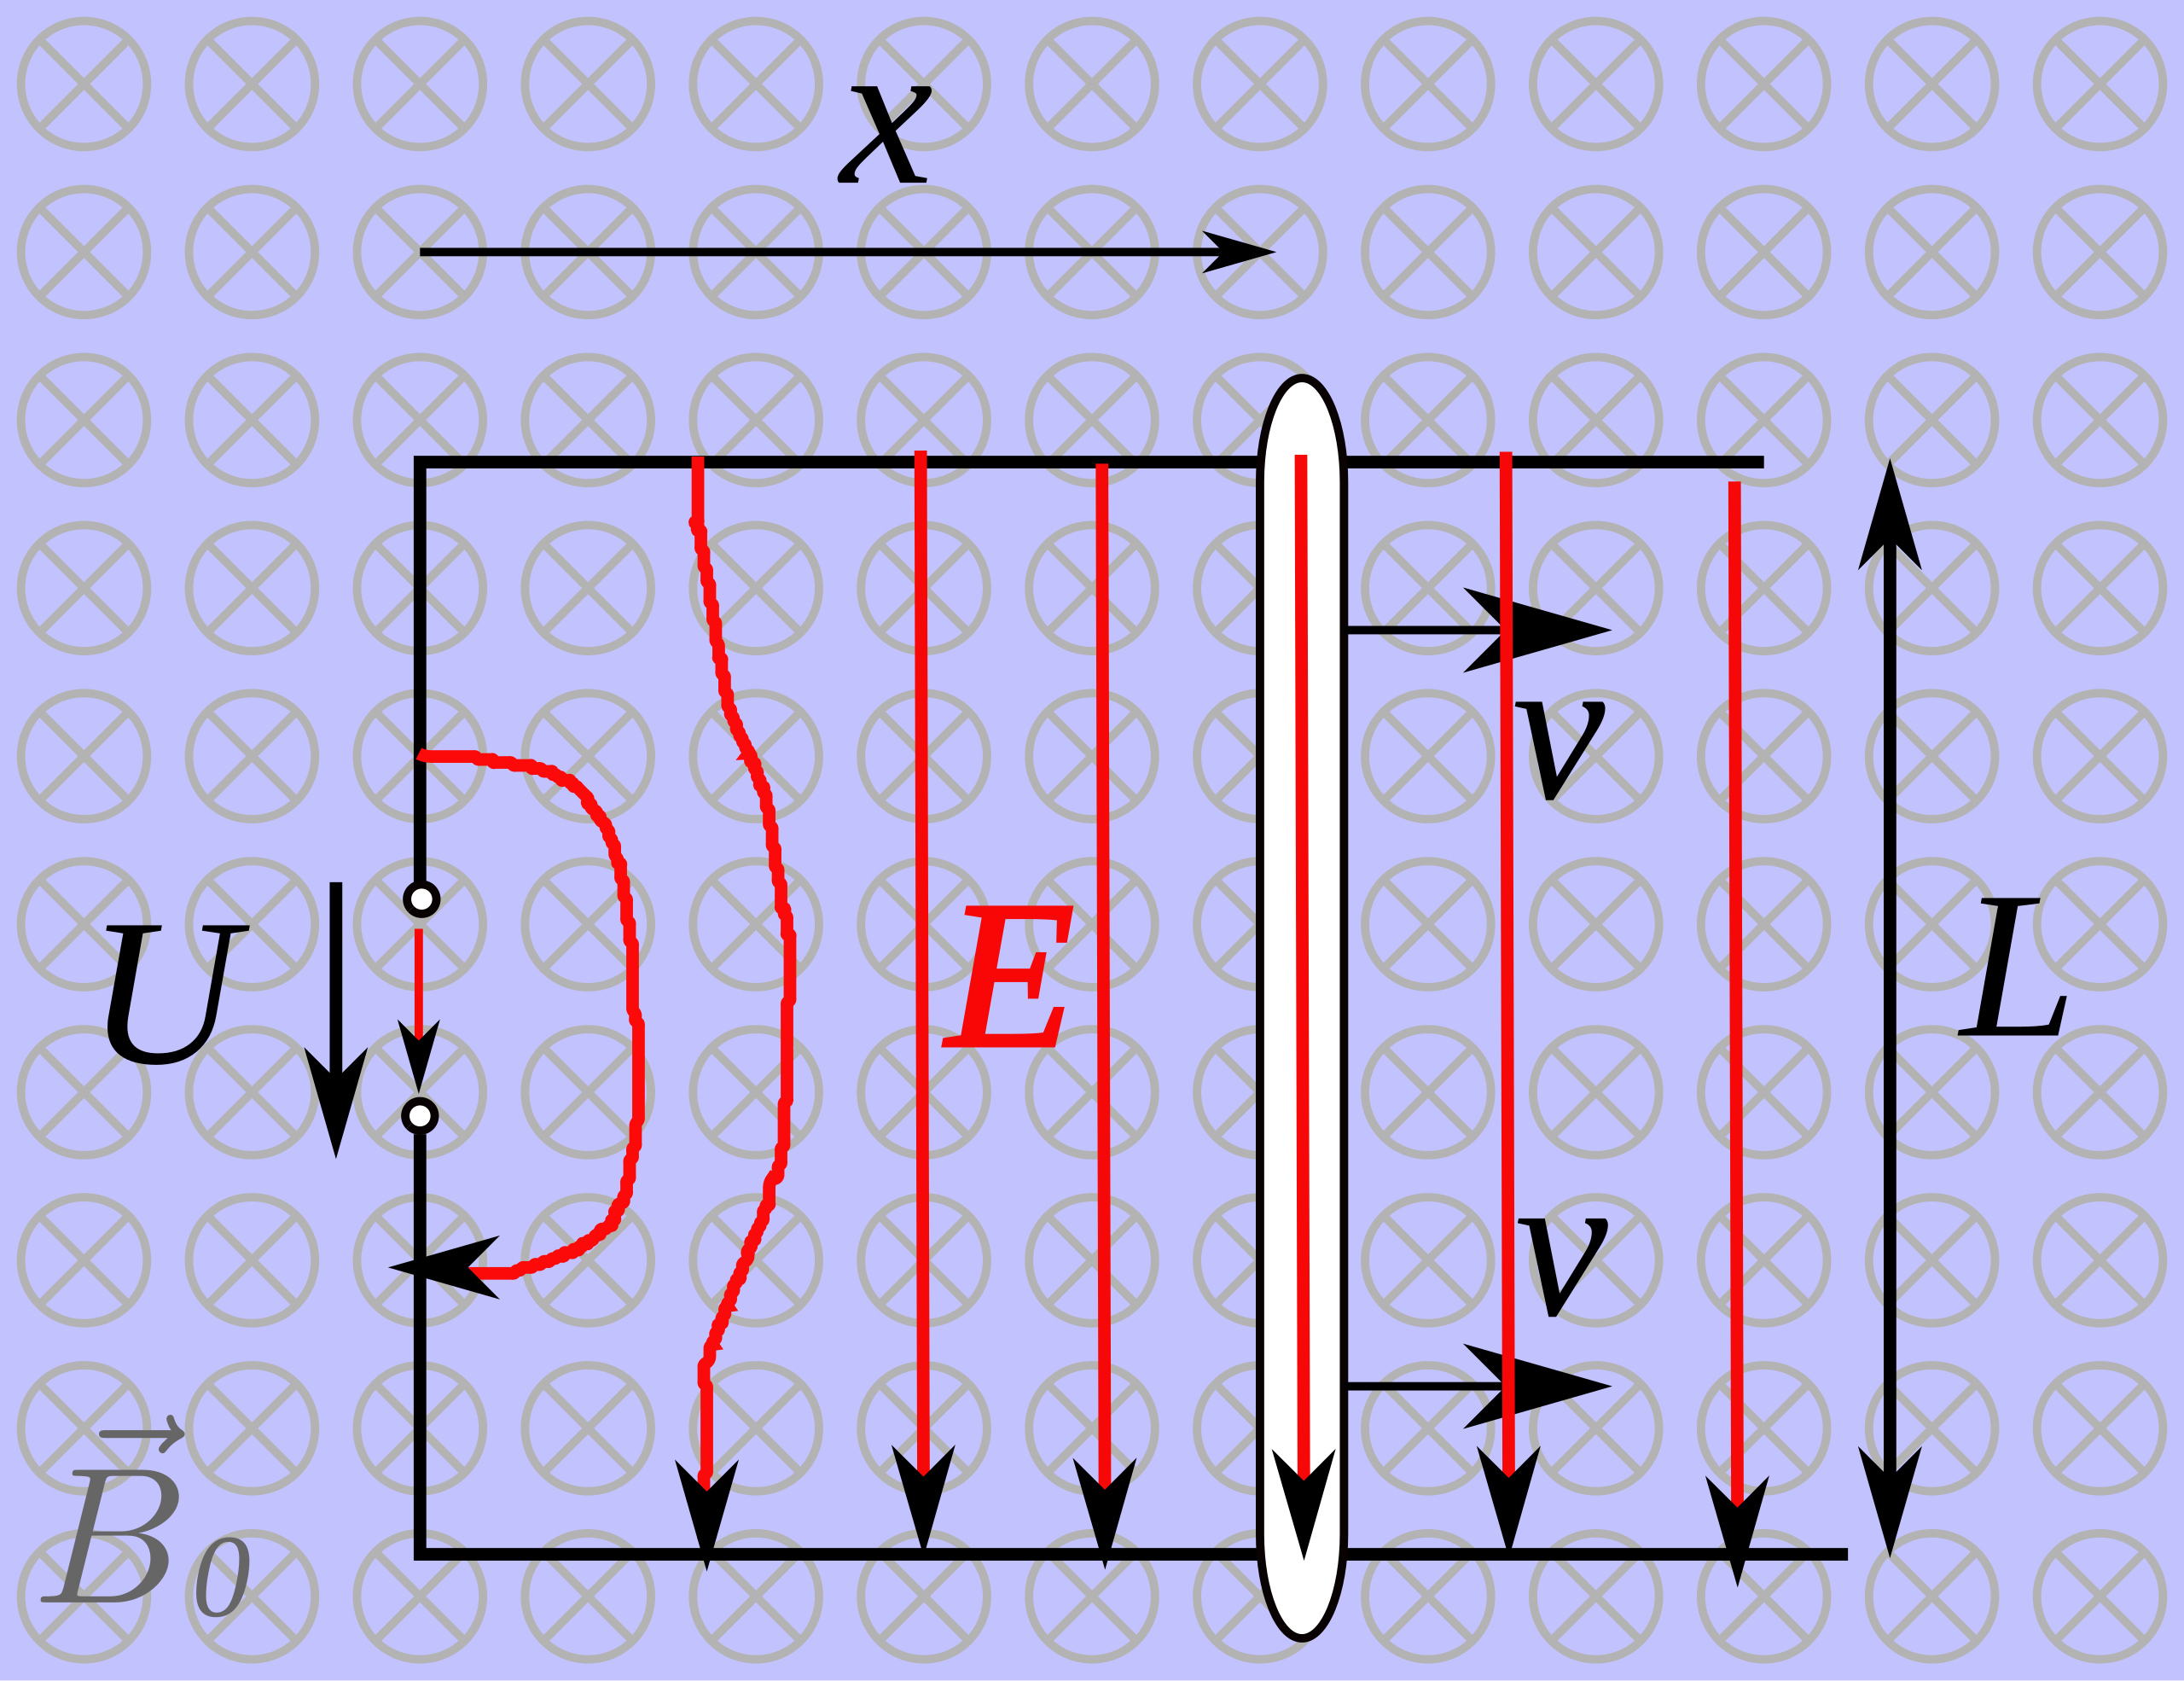
\includegraphics[width=5cm]{Bilder/Bewegter_Leiter_im_Feld-Feldlinienbild.svg}
		\item Abb. 2 unter \url{https://www.leifiphysik.de/elektrizitaetslehre/elektromagnetische-induktion/grundwissen/induktion-durch-aenderung-der-winkelweite}
	\end{enumerate}
	Wodurch unterscheiden sich die Darstellungen 1 bis 7? Können Sie diese hierarchisch ordnen? Welche Darstellung halten Sie für welche Zielgruppe für angemessen?
\end{uea}

Die Physik ist die Lehre von den Naturgesetzen. Ihre Methode ist die Modellbildung, um Phänomene in der Umwelt erklären und vorhersagen zu können. Die besten Modelle, die wir derzeit für die Beschreibung der Natur haben, sind unter anderem
\begin{itemize}
	\item die Allgemeine Relativitätstheorie für alle Phänomene auf großen Größenskalen,
	\item die Quantenmechanik für alle Phänomene auf kleinen Größenskalen und
	\item die Maxwell'schen Gleichungen zur Beschreibung elektromagnetischer Felder.
\end{itemize}
Diese Modelle sind hochkomplex und beruhen auf höherer Mathematik. Als Physiklehrkraft müssen Sie also vereinfachen!

\begin{figure}[hb]
	\centering
	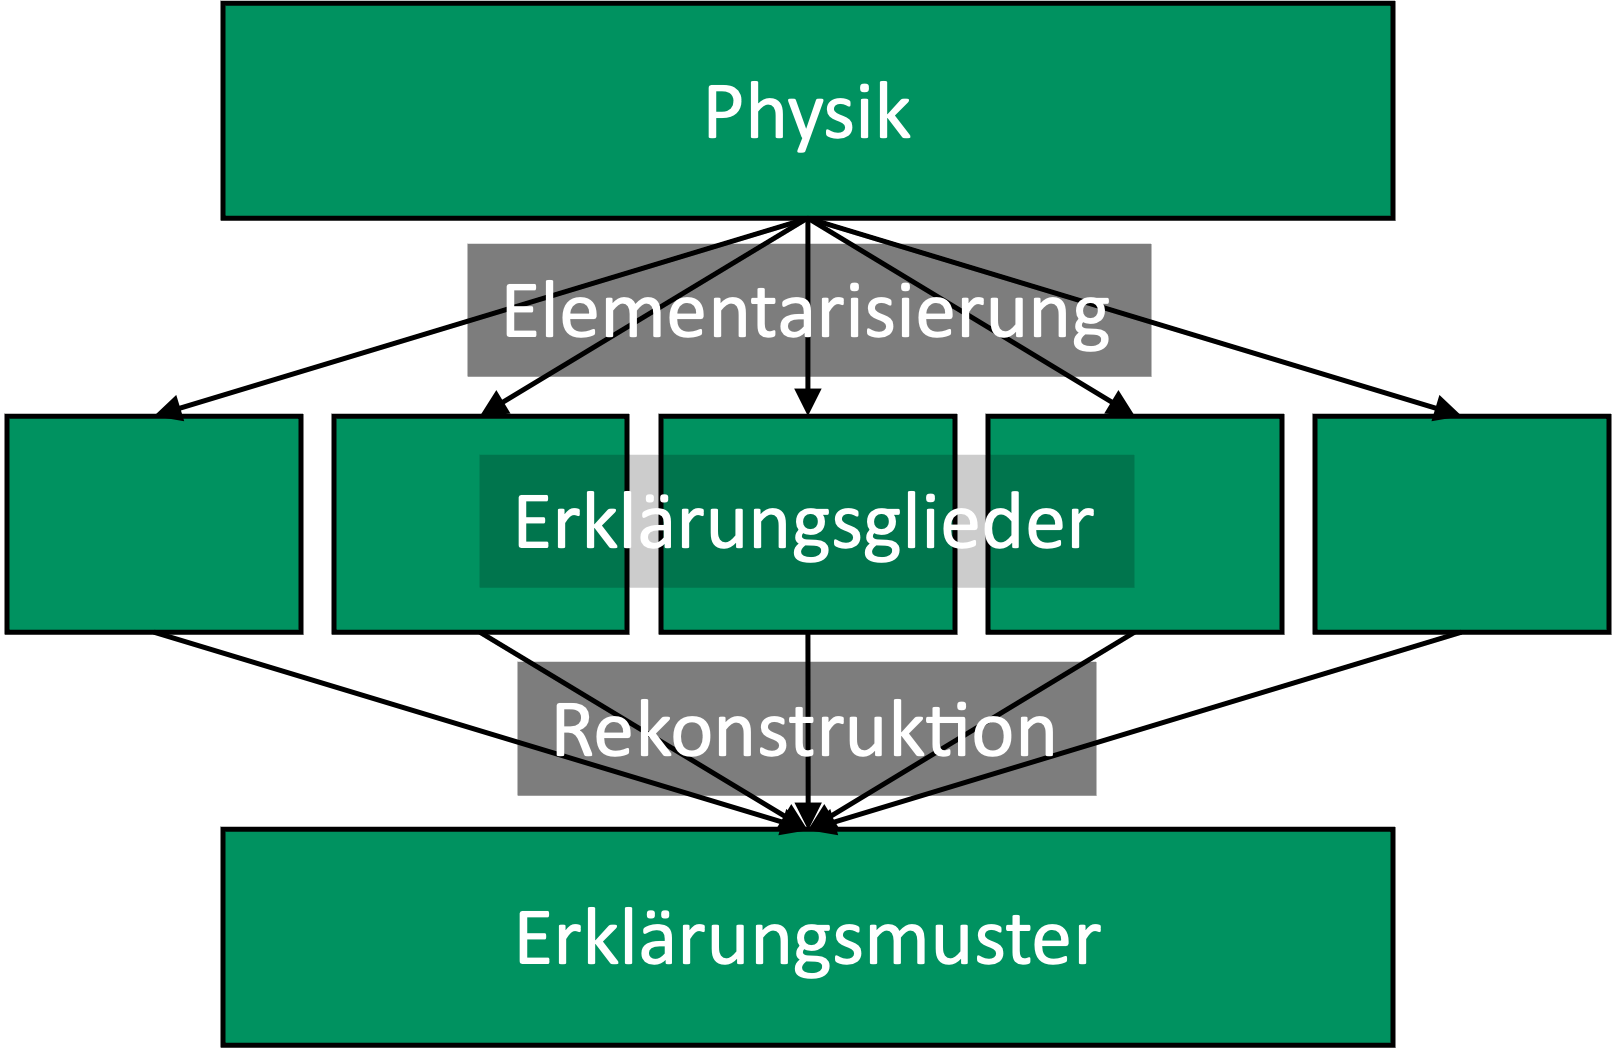
\includegraphics[width=7cm]{Bilder/elementarisierung}
	\caption{Elementarisierung und didaktische Rekonstruktion}\label{fig:elementarisierung}
\end{figure}

\mip
Wir wollen unter \textbf{Elementarisierung} oder \textbf{Didaktischer Reduktion} die \emph{fachlich zulässige Vereinfachung physikalischer Inhalte} verstehen. Das \emph{Zusammensetzen dieser Sinneinheiten zu einer Sachstruktur im Unterricht} nennen wir \textbf{Didaktische Rekonstruktion} ($\to$ Pestalozzis Traum in \cite[S. 158 f.]{KircherGirwidzHaussler1}). 


\bip

Betrachten wir ein
\begin{beisp}
	Verschiedene Elementarisierungsstufen des Ohm'schen Gesetzes.
	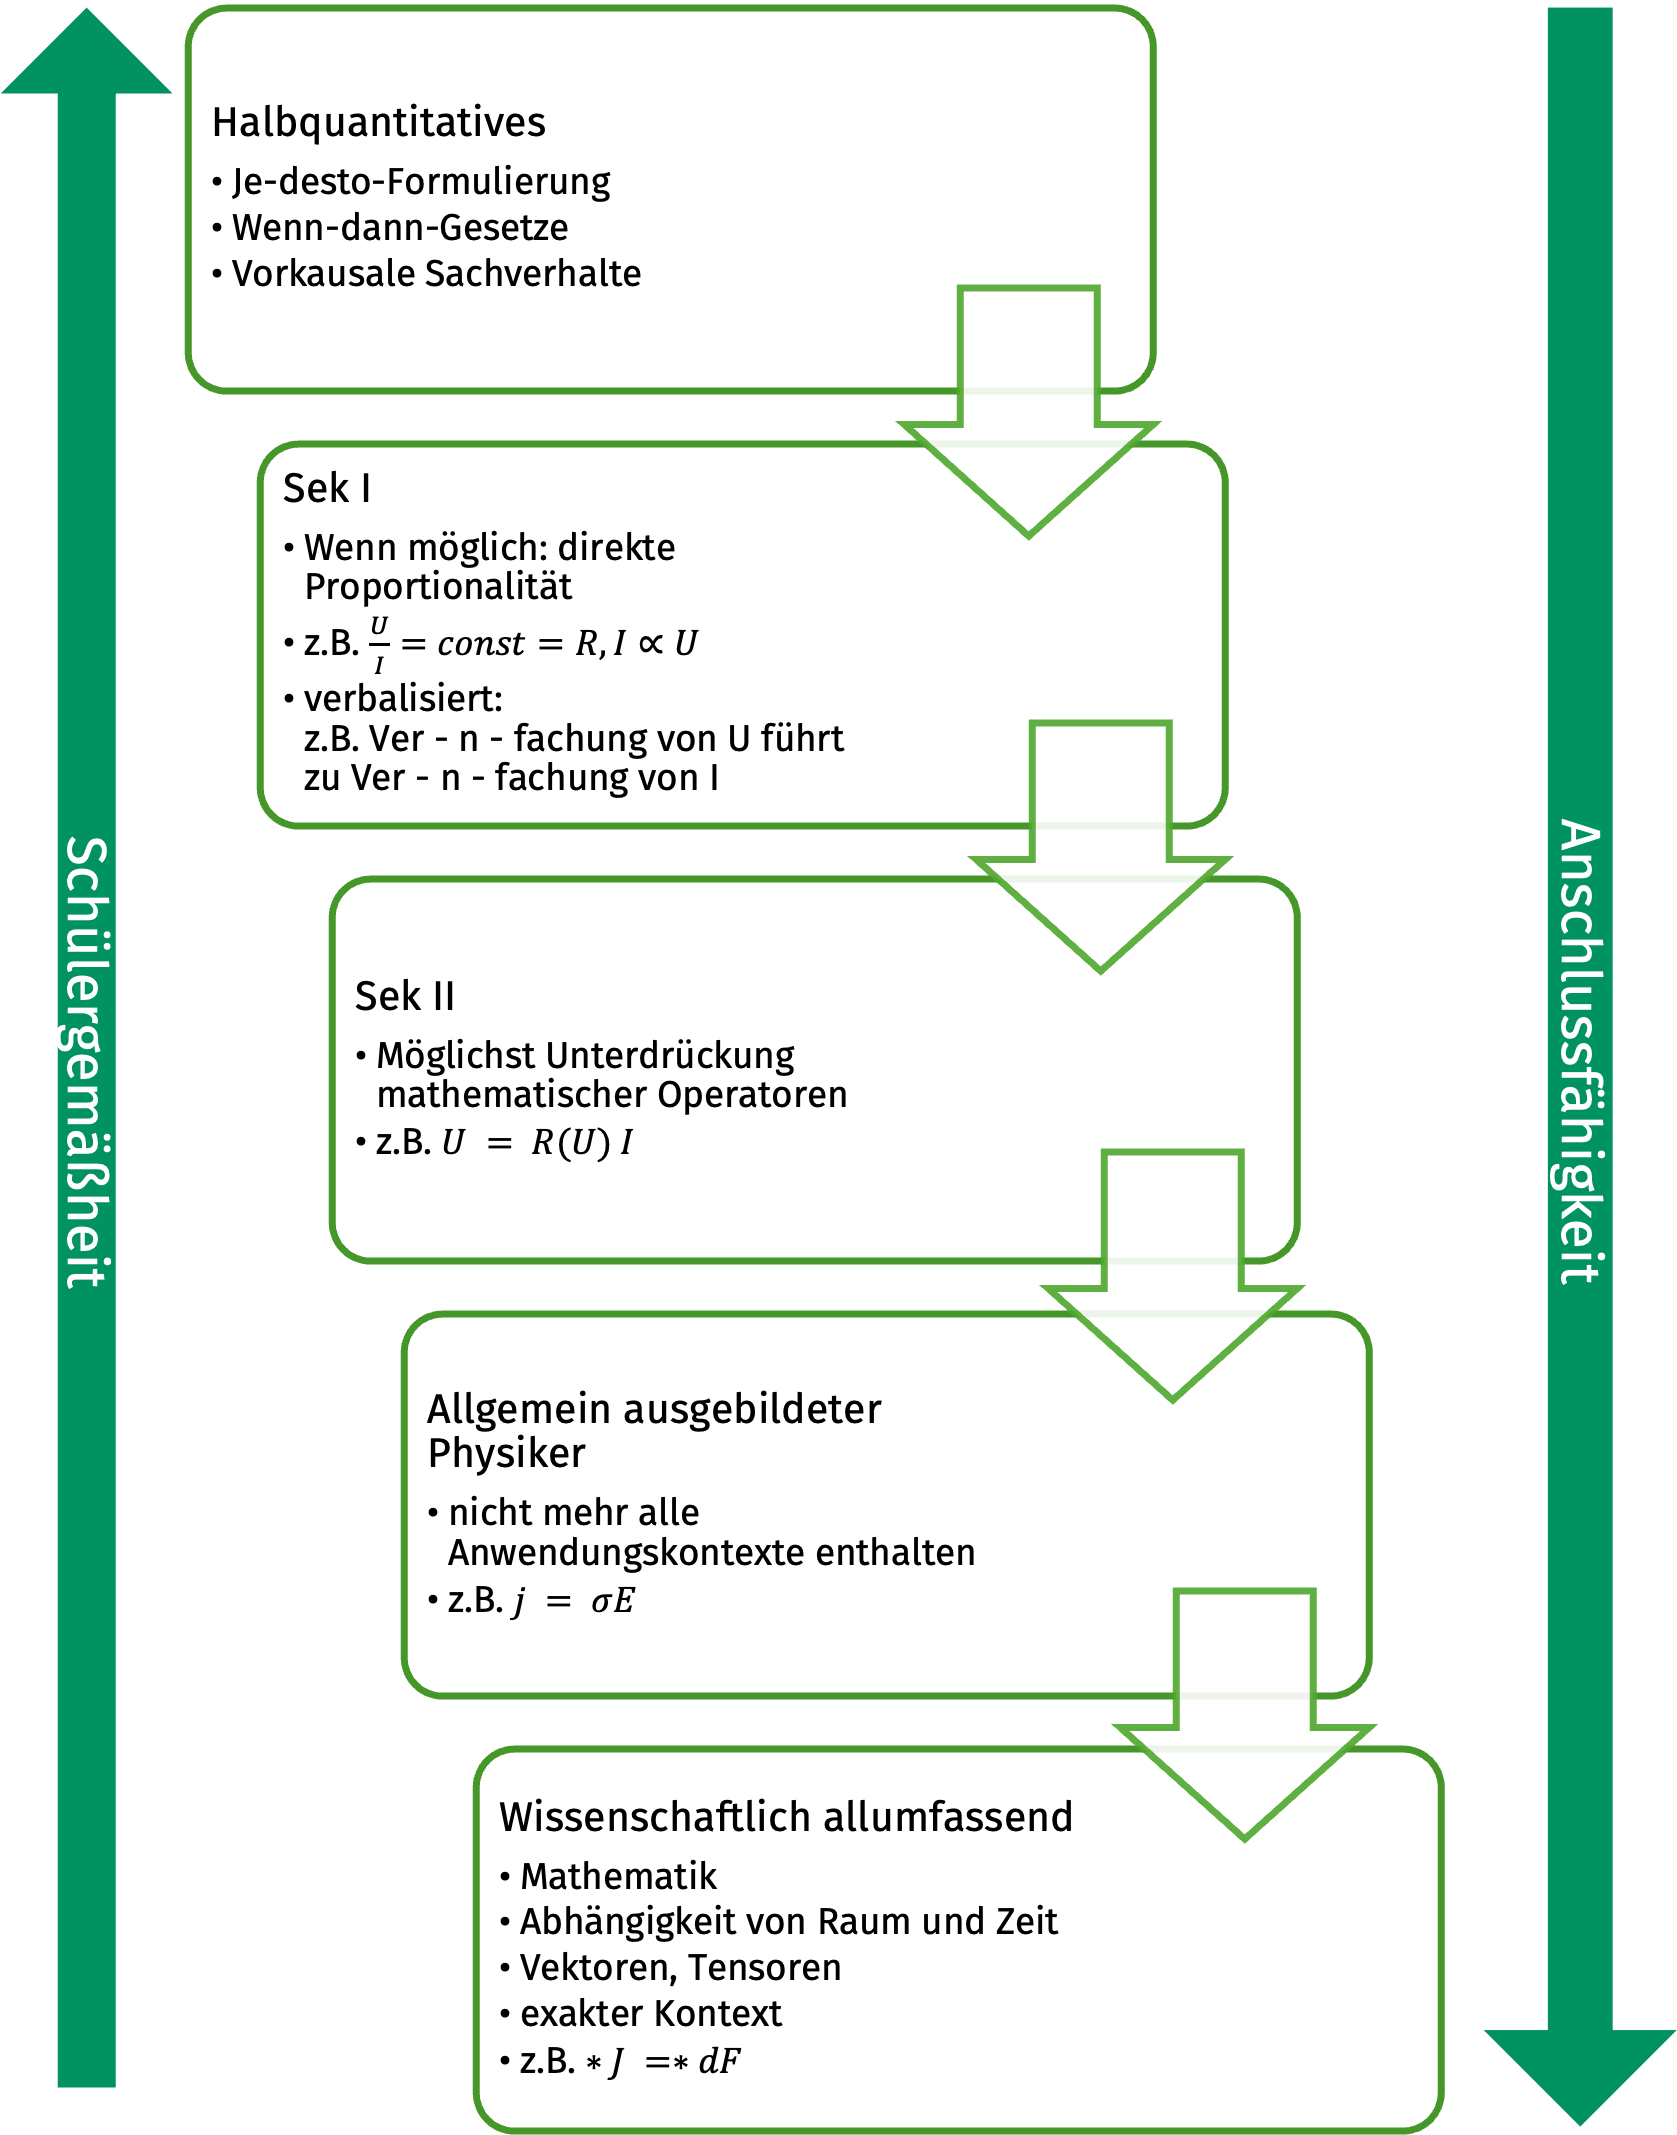
\includegraphics[width=\textwidth]{Bilder/ohm}
	
	Zentrales Element dieses Beispiels ist die Minimierung Reduktion des Quantitativen auf das Qualitative -- der Grad der Mathematisierung sinkt adressatengerecht, wobei die niedrigeren Elementarisierungsstufen hinreichend fachlich korrekt bleiben, um einen stetigen Anschluss zu gewährleisten. 
\end{beisp}

\subsection{Gütekriterien für Elementarisierungen}
\begin{itemize}
	\item \textbf{Adressatengerechtigkeit:} Das Anspruchsniveau muss für die Lernenden verständlich sein (z.~B. bedingt durch Alter, Jahrgangsstufe, Schulart, Vorerfahrung).
	\item \textbf{Sachgerechtigkeit:} Die Aufbereitung muss der Sache angemessen sein.
	\item \textbf{Fachgerechtigkeit:} Es müssen Darstellungsformen gewählt werden, die im Fach üblich sind.
	\item \textbf{Gültigkeit:} Bei der Elementarisierung darf keine Verf\"{a}lschung oder Verkehrung des Inhalts auftreten.
	\item \textbf{Anschlussfähigkeit:} Wer weiter lernt, soll das Gelernte nicht wieder verwerfen müssen. Bei weiterem Lernfortschritt soll die Elementarisierung im erweiterten Kontext weiterhin sinnvoll erscheinen.
	\item \textbf{Thematisierung und Transparenz:} Die Lehrkraft muss sich der Elementarisierung sowie ihrer Grenzen bewusst sein und die Lernenden darauf hinweisen.
\end{itemize}

\subsection{Typen der Elementarisierung}
Dies sind \"{U}berlegungen, die der Physikdidaktiker W.\ Jung,
Frankfurt, Anfang der Siebziger Jahre entwickelt hat:
Er unterscheidet --- orientiert an sachbezogenen Kategorien ---
die Typen der Elementarisierung wie
in der folgenden Liste aufgef\"{u}hrt.
Die Liste gibt Anregungen wieder. Im konkreten Beispiel ist eine
Einordnung bez\"{u}glich der Typen unter Umst\"{a}nden schwierig oder
mehrdeutig.
Bei einigen Typen kann man sich nicht des Eindrucks erwehren,
dass sie eigentlich nicht mehr den Kern der anfangs
gegebenen Definition treffen.

\begin{enumerate}
	\item \textbf{Reduktion vom Quantitativen auf das Qualitative:} Dies bedeutet im wesentlichen ein Zur\"{u}ckfahren des Grades der Mathematisierung ($\to$ obiges Beispiel).
	
	\begin{enumerate}
		\item
		Ausgangspunkt ist die wissenschaftlich-allumfassende Formulierung,
		wie sie vielleicht ein auf dem relevanten Gebiet spezialisierter
		Physiker zugrundelegt.
		\begin{itemize}
			\item
			Sie benutzt tieferliegende Begriffsbildungen der Analysis wie
			Grenzwerte, Integrale oder Ableitungen.
			
			\item
			Sie ber\"{u}cksichtigt raum-zeitliche Abh\"{a}ngigkeiten.
			Physikalische Gr\"{o}{\ss}en
			treten in Gestalt von Funktionen oder Feldern auf, meist wird
			dieses Abh\"{a}ngigkeit in den Formeln nicht mitgef\"{u}hrt,
			sondern nur stillschweigend vorausgesetzt.
			\item
			Sie ber\"{u}cksichtigt Richtungs- oder allgemeinere
			Trans\-for\-mations\-ab\-h\"{a}ngig\-kei\-ten (Vektoren, Tensoren).
			\item
			Der Kontext wird genau angegeben (Messvorschriften,
			G\"{u}ltigkeitsbereiche, Zuordnung zu klassischer,
			relativistischer oder Quanten-Physik).
		\end{itemize}
		
		\item Das Gesetz erh\"{a}lt eine wissenschaftliche Formulierung,
		die nicht mehr alle An\-wen\-dungs-Kon\-stella\-tio\-nen,
		wohl aber die physikalisch-prinzipielle Information, erfasst.
		Dies trifft in etwa das Niveau eines allgemein ausgebildeten
		Physikers.
		
		\item Das Gesetz wird nach wie vor formelm\"{a}{\ss}ig exakt, bei m\"{o}glichster
		Unterdr\"{u}ckung eines aufw\"{a}ndigen mathematischen
		Begriffsapparats, formuliert.
		Dies entspricht dem Niveau eines Studenten im Grundstudium
		oder Sch\"{u}lers der Sekundarstufe II (Kollegstufe).
		
		\item Wenn m\"{o}glich, werden Spezialfälle der direkten Proportionalit\"{a}t betrachtet.
		Dies ist in der Physik der Sekundarstufe I allgemein \"{u}blich.
		\begin{itemize}
			\item Quantitative Erfassung des konstanten
			Pro\-por\-tio\-na\-li\-t\"{a}ts\-fak\-tors
			\item Quotientengleichheit
			\item Graphische Darstellung in einem Koordinatensystem
			Es ergibt sich eine Ur\-sprungs\-(Halb-)Gerade mit dem
			Proportionalit\"{a}tsfaktor als Steigung
			\item Verbale Formulierung: Ver-n-fachung einer Größe führt zu Ver-n-fachung der zweiten Größe.\\
		\end{itemize}
		
		Verwandte andere Zusammenh\"{a}nge sind die der indirekten,
		der quadratischen, der quadratisch-reziproken Proportionalit\"{a}t
		oder der des logarithmischen Zusammenhangs.
		
		\item Je-desto-Gesetz (halb-quantitativ), üblich in den ersten Physik-Jahren.
		
		\mip
		Vorsicht: Eine Je-desto-Formulierung suggeriert eine direkte
		Proportionalit\"{a}t, obwohl vielleicht tats\"{a}chlich nur ein allgemeinerer
		nichtlinearer Zusammenhang vorliegt.
		
		\item
		Wenn-dann-Gesetz: Hier wird nur noch das Vorliegen eines kausalen
		Zusammenhangs dokumentiert: Wenn man A verändert, so ändert sich auch B.
	\end{enumerate}
	
	\item \textbf{Idealisierung:} Dies ist im wesentlichen eine Vernachl\"{a}ssigung von
	,,St\"{o}rungen'' oder von Kontexten, die in der Realit\"{a}t vorhanden,
	f\"{u}r das Verst\"{a}ndnis aber nicht zwingend notwendig sind.
	
	Idealisierung ist als eine wesentliche
	Erkenntismethode der Physik selbst Lerninhalt.
	So ist beispielsweise die durch die Vernachl\"{a}ssigung von
	Reibung gegebene Idealisierung beim Tr\"{a}gheitssatz wohl eher der
	Bestandteil eines Lernziels als eine gelungene
	Elementarisierung.
	
	\mip
	\begin{beisp}
		Vernachl\"{a}ssigung \dots
	\begin{itemize}
		\item
		der Reibung oder des Luft,,widerstands'',
		\item
		des Auftriebs in Luft (vgl.\ Kleiderb\"{u}gelwaage zum Nachweis
		des Gewichts von Luft),
		\item
		des Eigengewichts von Ger\"{a}teteilen (Rollen beim Flaschenzug,
		Feder beim Kraftmesser, Fl\"{u}s\-sig\-keit bei hydraulischer
		Presse,\dots) ($\to$ Ideale Kraftwandler),
		\item
		des Innenwiderstands von Messger\"{a}ten und damit des Spannungsabfalls
		an ihnen oder des Stromflusses in ihnen,
		\item
		Innenwiderstand von Stromquellen (Unproblematisch bei Netzger\"{a}ten,
		problematisch bei Haushalts\-batterien),
		\item
		der Belastung eines Potentiometers,
		\item
		von Linsenfehlern ($\to$ Ideale Linse),
		\item
		der Dispersion des Lichts,
		\item
		des W\"{a}rmeaustauschs eines Kalorimetergef\"{a}{\ss}es
		($\to$ Ideal isolierend),
		\item
		Energie- bzw.\ Leistungsverlusten bei Energiewandlern
		($\to$ Idealer Transformator),
		\item
		des Wellencharakters des Lichts: Dies f\"{u}hrt auf die geometrische Optik,
		\item
		von Auswirkungen tieferliegender physikalischer Theorien,
		beispielsweise von relativistischen oder Quanten-Effekten,
		\item
		der Richtungsabh\"{a}ngigkeit der Lorentzkraft: Es wird nur der Fall
		,,Bewegung $\perp$ Magnetfeld'' betrachtet,
		\item der Masse eines (beschleunigenden) Zuggewichtsst\"{u}cks
		(beispielsweise bei der Erarbeitung des 2.\ Newton'schen Gesetzes).
	\end{itemize}
	\end{beisp}
	
	\item \textbf{R\"{u}ckgriff auf historische Entwicklungsstufen}
	
	\mip
	\begin{beisp}
	\begin{itemize}
		\item Fr\"{u}here Festlegungen von physikalischen Einheiten und Naturkonstanten (Urmeter, Sonnentag, Lichtgeschwindigkeit, Kelvin).
		\item Die grunds\"{a}tzlich vorhandene M\"{o}glichkeit, akustische Signale
	in elektrische Signale umzuwandeln, l\"{a}sst sich einfacher anhand des 	Kohlek\"{o}rnermikrofons
	als anhand von Kondensator- oder Spulenmikrofonen aufzeigen.
		\item Atommodelle: Thomson --- Rutherford ($\to$ Mittelschule) ---
	Bohr --- Quantenmechanik.
	\end{itemize}
	\end{beisp}
	
	
	\item \textbf{Generalisierung}
	Allgemeing\"{u}ltige Aussagen sind ,,einfacher'' als spezielle Aussagen!
	
	\mip
	\begin{beisp}
	\begin{itemize}
		\item Alle Metalle leiten den elektrischen Strom.
		\item Alle festen und fl\"{u}ssigen K\"{o}rper dehnen sich bei Erw\"{a}rmung aus.
		\nip
		Beachte die Gegenbeispiele: Wasser (Anomalie im Temperaturbereich
		\SIrange{0}{4}{\celsius}), Quecksilber, Bismut, Gummi.
		\item Alle Metalle haben bei einer erh\"{o}hten Temperatur einen h\"{o}heren
		spezifischen Widerstand (Aber beachte die Halbleiter).
		\item
		Die vielen Einzeltheorien zur Beugung an optischen
		Hindernissen (Einzelspalt, Doppelspalt, Mehrfachspalt, Gitter,
		Lochblende,\dots) lassen sich in einer einzigen Theorie
		(mit dem mathematischen Konzept der Fouriertransformation
		im Hintergrund) zusammenf\"{u}hren.
	\end{itemize}
	\end{beisp}

	
	Letztlich ist Generalisierung eine der wesentlichen Triebkr\"{a}fte
	f\"{u}r den physikalischen Erkenntnisprozess: Einzelkonzepte zur Deutung
	von Teilaspekten der Welt werden zu umfassenderen Gesamtkonzepten
	vereint, die diese Aspekte als Spezialf\"{a}lle miterfassen.
	In dieser Hinsicht bringt es die Generalisierung mit sich,
	dass zwar die Aussagen immer einfacher und ,,sch\"{o}ner'' werden,
	die zugrundeliegenden mathematischen Rahmenkonzepte aber
	aufwendiger und komplexer.
	
	\mip
	\begin{beisp}
	\begin{itemize}
		\item Die Newton'schen Gleichungen bilden die Grundlage der gesamten
		Mechanik.
		\item Die Maxwell'schen Gleichungen enthalten alle Gesetzm\"{a}{\ss}igkeiten
		der klassischen Theorie des Elektromagnetismus und der Wellenoptik.
		\item Die vier Haupts\"{a}tze der W\"{a}rmelehre enthalten das
		Gesamtsystem der (ph\"{a}nomenologischen) Thermodynamik.
		\item
		Die Grand Unified Theory (GUT) dr\"{u}ckt das (in weiten Teilen)
		erfolgreiche Bestreben aus, die vier physikalischen Grundkr\"{a}fte
		als Ausgestaltung einer einzigen ,,Urkraft'' zu deuten.
		(Stichwort: Weltformel).
		\item
		Die Gesetze \"{u}ber das ideale Gas von
		Gay-Lussac, Boyle-Marriotte und Amontons k\"{o}nnen zu der einen
		Allgemeinen-Gas-Gleichung generalisiert werden.
		\item
		Goldene Regel der Mechanik.
		\item
		Energieerhaltungssatz.
	\end{itemize}
	\end{beisp}
	
	\item { \it Partikularisierung }
	Nur ein Teilaspekt der Sachstruktur wird beleuchtet.
	Ein physikalisches Konzept wird nur innerhalb eines Teilgebiets der
	Physik betrachtet.
	
	\mip
	\begin{beisp}
	\begin{itemize}
		\item Statischer Kraftbegriff (Ursache von Verformungen) statt dynamischer
	Kraftbegriff (Bewegungs\"{a}nderung).
		\item Energie wird nur in der Mechanik behandelt.
	\end{itemize}	
	\end{beisp}

	
	Vgl.\ auch weiter unten: Aspektierung.
	
	\item \textbf{Reduktion einer begrifflichen Differenzierung}
	
	\mip
	\begin{beisp}
	\begin{itemize}
		\item Masse --- Gewichtskraft (in GS),
		\item Masse --- Stoffmenge,
		\item Begriff der W\"{a}rme:
		\begin{itemize}
			\item Schule: nicht substanzlich aber mengig,
			\item Wissenschaft: Gegensatz zu Arbeit,
			\item ,,W\"{a}rme steigt nach oben'',
		\end{itemize}
		\item ferromagnetisch --- magnetisch,
		\item Zentripetalkraft --- Zentrifugalkraft,
		\item Celsius --- Kelvin,
		\item Gl\"{u}hlampe --- Gl\"{u}hbirne.
	\end{itemize}
	\end{beisp}
	
	Hochproblematisch ist eine Verschleierung des Unterschieds von:
	\begin{itemize}
		\item W\"{a}rme(menge) --- Temperatur,
		\item Stromst\"{a}rke --- Spannung,
		(vgl.\ das oft verwendete Wort: Stromspannung),
		\item Kraft --- Arbeit/Energie --- Leistung,
		\item Geschwindigkeit --- Beschleunigung.
	\end{itemize}
	
	Gegebenenfalls sollte nur der eine jeweils zutreffende Begriff tats\"{a}chlich gebraucht werden.
	
	\item \textbf{Reduktion auf das Elementare oder Prinzipielle}
	\begin{itemize}
		\item Anstelle eines Generatormodells wird eine Leiterschleife oder
		-schaukel eingesetzt.
		\item Superpositionsprinzip: Anstelle der allgemeinen
		dreidimensionalen Situation wird die ein- oder zweidimensionale
		Situation betrachtet (z.B.\ in der Mechanik).
	\end{itemize}
\end{enumerate}
\subsection{Verwandte didaktische Begriffsbildungen}

\begin{enumerate}
	\item \textbf{Animistische Sprechweise:} Bilder aus der belebten
	Welt werden auf die unbelebte Welt \"{u}bertragen.
	
	\mip
	\begin{beisp}
	\begin{itemize}
		\item Elektronen zw\"{a}ngen sich durch den Draht.
		\item Zink entrei{\ss}t dem Kohlenstoff ein O-Atom.
		\item Das Tee\-glas gew\"{o}hnt sich an die Temperatur.
		\item Bei C-H-Verbindungen: ,,Eltern und ihre Kinder''.
	\end{itemize}
	\end{beisp}
	
	\item \textbf{Antropomorphierung (Vermenschlichung)}
	Der Sch\"{u}ler setzt sich selbst k\"{o}rperlich oder gedanklich in die
	Situation hinein.
	
	\begin{beisp}
	\begin{itemize}
		\item Bewegungsspiele zur Modellierung
		astronomischer Bewegungsabl\"{a}ufe.
		\item Dann steigen die Regentr\"{o}pfchen immer h\"{o}her und r\"{u}cken immer
		n\"{a}her zusammen, weil sie frieren.
		\item Ladungsm\"{a}nnlein wandern im Kreis und geben in Eimerchen
		mitgebrachte Energie ab.
	\end{itemize}
	\end{beisp}
	
	H\"{a}ufig findet man Anthropomorphierung zur Darstellung von
	Vorg\"{a}ngen im menschlichen K\"{o}rper.
	Bekannt sind eher kabarettistische Umsetzungen durch Otto
	oder Woody Allan.
	
	\item \textbf{Reduktion durch Aspektierung}
	
	\begin{beisp}
	\begin{itemize}
		\item  Ein Regenbogen wird lediglich nach Form,
		Sonnenstand, Reihenfolge der Farben beschrieben und nicht
		erkl\"{a}rt.
		\item Der abstrakte Energiebegriff wird lediglich in
		seinen \"{a}usserlich erfahrbaren Aspekten (Bindung an Materie, Energietr\"{a}ger)
		eingef\"{u}hrt.
		\item Der Spannungsbegriff wird lediglich als eine
		(zun\"{a}chst nicht hinterfragbare) Kenngr\"{o}{\ss}e von
		Stromquellen erfahren.
	\end{itemize}
	\end{beisp}
	
	\item \textbf{ \it Ver\"{a}nderung des (raumzeitlichen) Koordinatensystems des
	Betrachters}
	\begin{beisp}
	\begin{itemize}
		\item Grundschule: Die Sonne geht im Osten auf und im Westen unter.
		\item Nachempfinden der Weltalter-Zeitskalen durch das ,,Eintagesweltmodell'',
		\item Nachempfinden der astronomischen L\"{a}ngenskalen durch Einf\"{u}hrung eines
		Ma{\ss}stabes (Erde ist Stecknadelkopf, Sonne ist Apfel,\dots)
	\end{itemize}
	\end{beisp}
	
\end{enumerate}

\begin{uea}
	Erarbeiten Sie verschiedene Elementarisierungsstufen des Hooke'schen Gesetzes!
\end{uea}

\subsection{Elementarisierung erkennen}
Häufig werden Sie nicht selber elementarisieren -- diese Aufgabe übernehmen zum Beispiel Schulbuchverlage für Sie. Dennoch gelten die oben genannten Gütekriterien fort, insbesondere die personalen. Sie müssen also weiterhin für deren Einhaltung sorgen. \begin{itemize}
	\item Moment! So einfach ist es doch nicht!
	\item Hmm, das stimmt doch nicht ganz\dots
	\item Das Modell erklärt diesen Effekt ganz gut, aber \dots
	\item Halt! Eigentlich ist es komplizierter!
\end{itemize}
Haben Sie einen dieser Eindrücke, dann aktivieren Sie Ihr Fachwissen und machen Sie sich klar, ob die Gütekriterien erfüllt sind oder ob Sie das Material modifizieren müssen, um es bedenkenlos im Unterricht verwenden zu können.

%\subsection{Weitere Beispiele}
%\begin{itemize}
%\item
%Hebelgesetz: Hier kann eine Elementarisierung auf verschiedensten
%inhaltlichen Ebenen durchgef\"{u}hrt werden:
%\begin{itemize}
%\item Zahl der angreifenden Kr\"{a}fte,
%\item zweiarmiger --- einarmiger Hebel,
%\item Winkel zwischen Kraftlinie und Kraftarm,
%\item eben oder r\"{a}umliche Situation,
%\item Schwerer Hebel,
%\item Realisierung des Hebelk\"{o}rpers (Stange, Scheibe, beliebig,
%bzgl.\ Sichtbarkeit des Kraftarms.)
%\end{itemize}
%
%\item Auftrieb,
%\item Begriff der Beschleunigung.
%\item Abh\"{a}ngigkeiten der Pendelfrequenz (vgl.\ \cite[S.\ 56,
%Piaget/Inhelder-Versuch]{Joerger}).
%\item Brechung,
%\item Spezifischer Widerstand,
%\item Induktionsgesetz: Vgl.\ STX, H97/3.
%
%\end{itemize}


\bip\bip
\subsection{Didaktische Rekonstruktion nach Kattmann}

Das Modell der \textit{Didaktischen Rekonstruktion} nach \textcite{Kattmann} ist ein Konzept zur Gestaltung von Lernprozessen, das wissenschaftliche Inhalte verst\"{a}ndlich und zug\"{a}nglich f\"{u}r Lernende aufbereitet. Dieser Ansatz kombiniert fachwissenschaftliche, fachdidaktische und lernpsychologische Perspektiven, um Unterrichtsinhalte optimal zu strukturieren.
\bip
Der Prozess der didaktischen Rekonstruktion umfasst drei wesentliche Schritte:
\begin{enumerate}
    \item \textbf{Fachliche Kl\"{a}rung}: Pr\"{a}zise Analyse und Strukturierung der relevanten wissenschaftlichen Konzepte, um die inhaltliche Korrektheit sicherzustellen.
    \item \textbf{Erfassung von Sch\"{u}lervorstellungen}: Untersuchung der Vorkenntnisse und Vorstellungen der Lernenden, um m\"{o}gliche Fehlkonzepte zu identifizieren.
    \item \textbf{Didaktische Strukturierung}: Entwicklung geeigneter Methoden und Materialien auf Grundlage der vorherigen Schritte, um die Lerninhalte verst\"{a}ndlich und effektiv zu vermitteln.
\end{enumerate}

Das Ziel der didaktischen Rekonstruktion ist es, die Kluft zwischen wissenschaftlichem Wissen und den Lernvoraussetzungen der Sch\"{u}ler zu \"{u}berbr\"{u}cken und den Lernprozess zu erleichtern.



%------------------------------------------------------------------------------------------------------------
\bip\bip
\section{Analogien und Modelle im Physikunterricht}


%----------------------------- Analogien -------------------------------------------------


\subsection{Analogien}

\begin{quote}
Jede Aufgabe, die ich l\"{o}ste, wurde zu einer Regel, die
sp\"{a}ter zur L\"{o}sung anderer Aufgaben diente.
\q\q R\`ene Descartes (31.3.1596 -- 11.2.1650)
\end{quote}

\begin{quote}
Analogien sind meine zuverl\"{a}ssigsten Lehrmeisterinnen ---
vertraut mit allen Geheimnissen der Natur.
\q\q Johannes Kepler (1571 -- 1630)
\end{quote}

\pph{Definition} Weisen zwei verschiedene (evtl.\ fachfremde) Inhalte gleiche
Strukturen auf, so spricht man von einer \textit{Analogie} in diesen
Inhalten.

\bip
Ist der eine Inhalt (A) gegen\"{u}ber dem anderen Inhalt (B)
\begin{itemize}
\setlength{\itemsep}{0mm}
\item
lebensn\"{a}her,
\item
anschaulicher (den Sinnen unmittelbarer zug\"{a}nglich),
\item
elementarer (vgl.\ Begriff der Elementarisierung),
\item
besser verstanden oder erforscht, \q\q oder
\item
st\"{a}rker (alltags-)pr\"{a}sent,
\item
in der Pr\"{a}sentation sicherer, kosteng\"{u}nstiger oder schneller,
\end{itemize}

so stellt Inhalt (A) ein \textit{Modell} f\"{u}r den Inhalt (B) dar.

\bip
Analogien sind also ein effektives p\"{a}dagogisches Werkzeug im Physikunterricht, das dabei hilft, komplexe oder abstrakte Konzepte verst\"{a}ndlicher zu machen, indem sie mit vertrauten Situationen oder Strukturen verglichen werden. Durch den Einsatz von Analogien k\"{o}nnen Lernende neue Konzepte auf Basis von bereits vorhandenem Wissen leichter begreifen. Analogien sind ein wesentlicher ``Mechanismus'' f\"{u}r die Vernetzung eines Denksystems. ($\to$ Ausubel: Sinnvoll \"{u}bernehmender Unterricht). Analogien f\"{o}rdern insbesondere das kritische Denken, indem sie Lernende anregen, \"{u}ber Gemeinsamkeiten und Unterschiede zwischen den verglichenen Konzepten nachzudenken.

\bip
Es ist jedoch wichtig, dass Lehrkr\"{a}fte die Grenzen und m\"{o}glichen Missverst\"{a}ndnisse von Analogien im Blick behalten. Nicht alle Aspekte eines bekannten Systems k\"{o}nnen auf das neue Konzept \"{u}bertragen werden, weshalb Analogien sorgf\"{a}ltig ausgew\"{a}hlt und erl\"{a}utert werden sollten.

\bip
\pph{Klassifizierung von Analogien}

\begin{itemize}
\item{\textbf{Strukturelle Analogien:} Diese betonen die \"{a}hnlichkeit in der Struktur zwischen zwei unterschiedlichen Systemen, wie z.B. die Analogie zwischen einem elektrischen Stromkreis und einem Wasserkreislauf.}
\item{\textbf{Funktionale Analogien:} Diese fokussieren auf die \"{a}hnliche Funktion oder das Verhalten zweier Systeme, wie z.B. die Analogie zwischen der Bewegung von Planeten um die Sonne und Elektronen um einen Atomkern.}
\item{\textbf{Bildhafte Analogien:} Diese nutzen leicht verst\"{a}ndliche Bilder oder Geschichten, um abstrakte Konzepte zu veranschaulichen, wie z.B. das Bild einer mit Murmeln gef\"{u}llten Kiste zur Veranschaulichung von Gasdruck.}
\end{itemize}

\pph{Beispiele f\"{u}r Analogien}

\begin{center} \small
\begin{tabular}{ p{5cm} @{\q --- \q } p{5cm} }
Mechanische Schwingungen & Elektromagnetische Schwingungen \\

Reflexion von Lichtstrahlen an Grenzfl\"{a}chen
& Reflexion von K\"{o}rpern an W\"{a}nden  (Billard, Eishockey) \\

R\"{o}hrentechnik (B Vakuumdiode) & Halbleitertechnik (HL-Diode) \\

Fortbewegung (Translation) & Drehbewegung  (Rotation) \\

Planetensystem           & Bohr'sches Atom  \\

Schwingende Saite & Quantenmechanisches Atom \\

Hysterese bei magnetischen Stoffen (B weich -- hart) &
Hysterese bei Dehnung (Verformung) von Stoffen (B weich -- hart) \\

Reihen- und Parallelschaltung von Schraubenfedern &
Reihen- und Parallelschaltung von Widerst\"{a}nden \\
& Reihen- und Parallelschaltung von Kondensatoren \\

Elektrische Gr\"{o}{\ss}en & Magnetische Gr\"{o}{\ss}en
                      (vgl.\ Tabelle in \cite{Stoecker}) \\

Phasen\"{u}bergang & Auf/Absteigen einer Kugel im Galileithermometer \\

Sammellinse & Hohlspiegel \\
Zerstreuungslinse & W\"{o}lbspiegel \\
Gesetz \"{u}ber radioaktiven Zerfall &
Barometrische H\"{o}henformel \\
& Turbidimetrie (Tr\"{u}bungsmessung in Suspensionen) \\

Beugung von Licht & Beugung von Wasserwellen
\end{tabular}
\end{center}

\bip
Prominent sind die Analogien in den Transportph\"{a}nomenen

\bip
\begin{center} \scriptsize
\begin{tabular}{ |l || *{4}{l|}}
\hline
%\ST  
Name
&  Diffusion
&  W\"{a}rmeleitung
&  El.\ Leitung
&  Str\"{o}mung einer Fl\"{u}ssigkeit
\\ \hline
%\ST 
Gesetz von \dots
&  Fick
&  Fourier
&  Ohm
&  Navier-Stokes
\\ \hline
%\ST   
Transportiert wird \dots
&  chem.\ Stoff
&  Innere Energie
&  El.\ Ladung
&  Mech.\ Impuls
\\ \hline
\end{tabular}
\end{center}

Klassisches Beispiel einer im Unterricht instrumentalisierten
Analogie ist die zwischen
\begin{quote}
Elektrischem Stromkreis \q und \q Wasserstromkreis
\end{quote}
(Siehe Vorlesung: Elektrizit\"{a}t-Magnetismus).


%----------------------------- Modelle -------------------------------------------------
\subsection{Modelle}

\pph{Definition} Ein Modell in der Physik ist ein ideelles (gedankliches) oder materielles (gegenst\"{a}ndliches) Objekt, das als Ersatzobjekt f\"{u}r ein Original benutzt wird. Es ist eine Vereinfachung oder eine Veranschaulichung des Originals und damit der Wirklichkeit. In einigen Eigenschaften stimmt das Modell mit dem original \"{u}berein, in anderen nicht. Ein Modell ist weder richtig noch falsch, sondern nur f\"{u}r einen bestimmten Zweck geeignet oder nicht geeignet.

\mip
Aus erkenntnistheoretischer Sicht beinhaltet unser gesamtes Denken bzw.\ Wissen \"{u}ber Physik lediglich Modelle der Wirklichkeit, niemals die Wirklichkeit selbst. Die Physik als Wissenschaft arbeitet immer mit Modellen. Mit Hilfe von Modellen kann eine Elementarisierung ($\to$ Kap. \ref{Elementarisierung}) durchgef\"{u}hrt werden.  Modellbildung z\"{a}hlt zu den Schl\"{u}sselqualifiktionen des Physikers.

\mip
Ganz allgemein m\"{u}ssen Modelle (i) sachgerecht sein (Die ,,Ladungsm\"{a}nnlein'' sind ungeeignet); (ii) sch\"{u}lergerecht sein (Das quantenmechanische Atommodell ist f\"{u}r die SI zu abstrakt). 

\bip
\pph{Didaktische Funktionen von Modellen:}

\begin{itemize}
\item heuristische Funktion: Gewinnung neuer Erkenntnisse, Hypothesen testen, Modelle m\"{u}ssen in einem definierten Bereich Vorhersagen \"{u}ber das Original zulassen
\item Veranschaulichungsfunktion von Sachverhalten, Strukturen, theoretischen Konstrukten und Abl\"{a}ufen
\item Vereinfachungsfunktion; Modelle m\"{u}ssen das Original ad\"{a}quat und auf das Wesentliche reduziert abbilden. Modelle sind keine Kopie des Originals, d.h. nicht alle Modelleigenschaften stimmen mit dem Original ueberein
\item Funktion der Lern\"{o}konomie bzw. Denk\"{o}konomie - neue Infos k\"{o}nnen schneller aufgenommen und behalten werden 
\end{itemize}


\pph{Klassifizierung von Modellen:}
\mip
Die wissenschaftliche Klassifizierung von Modellen ist un\"{u}bersichtlich. Eine \"{U}bersicht ist in in diesem Artikel \footnote{Silke Michelskis-Seifert, Marco Thiele und Thilo W\"{u}nscher, PhyDid 1/4 (2005) S. 30-46} gegeben. Modelle k\"{o}nnen nach unterschiedlichen Gesichtspunkten klassifiziert werden:

\begin{enumerate}
\item{\it{Klassifizierung nach der Lern- oder Erkenntnisabsicht}}
\begin{itemize}
\item
Analogmodelle: Eine Analogie wird hergestellt.
\begin{itemize}
\item Ameisenhaufen f\"{u}r Brown'sche Molekularbewegung.
\end{itemize}

\item
\"{A}hnlichkeitsmodelle: Ma{\ss}st\"{a}bliche Verkleinerung bzw.\ Vergr\"{o}{\ss}erung,
\begin{itemize}
\item Flugzeug,
\item kleiner Motor,
\item Globus.
\end{itemize}

\item
Funktionsmodelle:  Aufbauprinzipien k\"{o}nnen herausgestellt
werden, dynamische Abl\"{a}ufe verlangsamt werden.
\begin{itemize}
\item Elektromaschinen,
\item Otto-Motor,
\item Dampfmaschine,
\item Zentralheizungsmodell,
\item Tellurium (Mechanisches Modell des Erde-Mond-Sonnensystems),
\item Hydraulische Presse.
\item Transformatormodell: Punktschwei{\ss}en, Induktionsofen.
\end{itemize}

\item
Strukturmodelle:
Darstellung von Strukturen von Gegenstandsbereichen:
\begin{itemize}
\item Teilchenmodell,
\item Gittermodell,
\item Molek\"{u}lmodelle, Kalottenmodelle f\"{u}r Molek\"{u}le.
\end{itemize}

\item
Theoretische Modelle:
\begin{itemize}
\item Atommodelle von Thomson, Rutherford, Bohr, Quantenmechanik.
\item Kosmologische Modelle
(Friedmann Universe, steady state,\dots).
\end{itemize}

\item
Black-Box-Modell: Ein physikalischer Inhalt, insbesondere ein
physikalisches Ger\"{a}t oder Messger\"{a}t, wird nur in seinen \"{a}u{\ss}eren
Eigenschaften und Funktionen, nur als Ph\"{a}nomen, erfasst.
Die inneren Eigenschaften oder Wirkzusammenh\"{a}nge sind nicht
oder nur sekund\"{a}r relevant, sie bleiben in der ,,Black Box''
verborgen. Der Lehrer(in) sollte jedoch die innere Struktur der ,,Black-Box''
kennen.

\mip
Beispiele:
\begin{itemize}
\item Im Alltag: Mikrowellenherd, Kaffeemaschine, Auto.
\item Die ,,Steckdose'' wird einfach als Spannungsquelle
erkannt und genutzt. Die Tatsache, dass das Netz der \"{o}ffentlichen
Stromversorgung mit all seinen Komponenten als Grundlage notwendig ist,
bleibt im Hintergrund.
\item Elektrische, elektronische Messger\"{a}te f\"{u}r Gr\"{o}{\ss}en aller Art.
      (el.\ Gr\"{o}{\ss}en, Temperatur,\dots).
\item Messverst\"{a}rker, Operationsverst\"{a}rker,
\item Computer
\item Hall-Sonde
\end{itemize}

\end{itemize}

\bip
\item{\it{Klassifizierung nach der Realisierung:}}
\begin{itemize}
\item
Gegenst\"{a}ndliche Modelle oder Modelle im engeren Sinne sind Apparaturen, die
einen technischen Zusammenhang durch prinzipielle
Hervorhebungen und Weglassungen {\bf statisch} verdeutlichen.
\begin{itemize}
\item Motormodell (in der Fahrschule),
\item Lichtleiter-Modell,
\item Zentralheizungsmodell der (klassischen) Schulphysik,
\item Kraftwerksmodelle,
\item Chemie: Kalottenmodelle von Molek\"{u}len. Sie waren entscheidend hilfreich bei der
Aufkl\"{a}rung der DNA-Struktur durch Watson und Crick
(Lesenswert: James Watson, Die Doppel-Helix, rororo-Sachbuch 6803, 1973.)
\item
Schaumstoffmodell f\"{u}r den Bitmetallstreifen.
\end{itemize}

\item
Ein Vorgang oder eine physikalische Gr\"{o}{\ss}e werden auf {\bf dynamische}
Weise verdeutlicht (Dynamische Modelle).
\begin{itemize}
\item Elektromaschinenmodelle (Elektromotor, Generator),
\item R\"{u}ttelapparat f\"{u}r die Maxwell'sche Geschwindigkeitsverteilung,
\item B\"{u}rstenmodell f\"{u}r Haft- und Gleitreibung,
\item Bierschaummodell f\"{u}r den radioaktiven Zerfall,
\item Kette aus Dominosteinen f\"{u}r Kettenreaktion (Vorsicht im
Zusammenhang mit Kernspaltung, die Analogie ist fast zu einfach),
\item ,,Gummiband-Modell''
der elektromagnetischen Wechselwirkungen (nicht so gl\"{u}cklich),
\item Kernspaltungs-Kettenreaktion: Mausefallen und Tischtennisb\"{a}lle.
\end{itemize}

\item
Modellexperimente
\begin{itemize}
\item
\"{U}berlandleitung,
\item
\textsc{und}, \textsc{oder} Schaltung,
\item
Verst\"{a}rkerschaltung,
\item
Schwei{\ss}ger\"{a}t, Induktionsofen.
\end{itemize}

\item
Ikonische Modelle: Vereinfachungen zur (mathematischen)
Beschreibung von Ph\"{a}nomenen (Idealisierung, Modellannahme)
\begin{itemize}
\item Lichtstrahl,
\item Massenpunkt,
\item Modell des idealen bzw.\ realen Gases,
\item Ebenes Modell eines Halbleiterkristalls.
\end{itemize}

\item
Symbolische Modelle:
\begin{itemize}
\item Schaltsymbole und Schaltbilder,
\item Mathematisch abstrakte Modelle: Gr\"{o}{\ss}en, Begriffe, Formeln.
\end{itemize}

\item
Reine Denkmodelle,
Anschauliche Vorstellungen von etwas Unanschaulichem:
\begin{itemize}
\item Atommodell,
\item Elektron als K\"{u}gelchen,
\item Tr\"{o}pfchen- oder Schalenmodell des Atomkerns,
\item Urnenmodell f\"{u}r die mathematische Kombinatorik.
\end{itemize}

\end{itemize}
\end{enumerate}

\mip
Letztlich sei darauf hingewiesen, dass die Modellbildung fester Bestandteil des Lehrplans in Bayern ist. Zur Kompetenzorientierung im Fach Physik hei{\ss}t es dort:\footnote{https://www.lehrplanplus.bayern.de/fachprofil/gymnasium/physik}

\begin{quote} ``Die Sch\"{u}lerinnen und Sch\"{u}ler kennen und erl\"{a}utern wesentliche naturwissenschaftliche Konzepte, Theorien und Verfahren, die sie zur Beschreibung und Erkl\"{a}rung von Experimenten und \emph{Modellen}, aber auch in allt\"{a}glichen Situationen nutzen. Auf dieser Grundlage w\"{a}hlen sie auch geeignete Experimente, \emph{Modelle} und mathematische Beschreibungen aus, um Problemstellungen zu Ph\"{a}nomenen und Sachverhalten aus innerfachlichen und alltagsbezogenen Anwendungsbereichen zu bearbeiten. Sie ber\"{u}cksichtigen dabei die entsprechenden G\"{u}ltigkeitsbereiche der ausgew\"{a}hlten \emph{Modelle} und Theorien bei der qualitativen und quantitativen Auswertung von Beobachtungen und Messergebnissen. \dots ''
\end{quote}


